


% ====================================================================
%+
% SECTION:
%    AGN_Disk_Extrinsic.tex
%
% CHAPTER:
%    AGN.tex
%
% ELEVATOR PITCH:
%    Using AGN microlensing to measure the size and structure of
%    accretion disks. Depends on well-sampled multi-filter light curves,
%    and a large sample of detected strongly-lensed AGN.
%
% AUTHORS:
%    Timo Anguita (@tanguita), Matthew O'Dowd
%-
% ====================================================================

\section{AGN Size and Structure with Microlensing}\label{sec:AGNMicrolensing}
\def\secname{\chpname:microlensing}\label{sec:\secname}

\credit{tanguita},
\credit{mattodowd}

Microlensing due to stars projected on top of individual
gravitationally-lensed quasar images produces additional magnification which can be used to probe the structure of the background high-redshift AGN.

The microlensing method is based on the fact that the variability amplitude depends on the quasar size relative to the Einstein radius of a star (projected into the source plane). By comparing the variability amplitudes at different wavelengths, we can determine the relative source sizes and test the predicted wavelength scaling: Assuming a thermal profile for accretion disks, sizes in different emission
wavelengths can be probed and as such, constraints on the slope of this
thermal profile can be obtained. Given the sheer number of lensed systems that LSST is expected to discover ($\sim8000$), this will allow us to stack systems for better
constraints and hopefully determine the {\it luminosity and redshift evolution
of the disk size and profile.} Due to the typical relative velocities of lenses,
microlenses, observers (Earth) and source AGN, the microlensing variation
timescales are between months to a few decades.


%Using the fact that the Einstein radii of stars in lensing galaxies
%closely match the scales of different emission regions in
%high-redshift AGNs (micro-arcseconds), analyzing microlensing induced
%flux variations statistically on individual systems allows us to
%measure ``sizes'' of AGN regions.


% --------------------------------------------------------------------

\subsection{Target measurements and discoveries}
\label{sec:\secname:targets}

Analysis of microlensing induced variability will allow the measurement of
accretion disk sizes $R_\lambda$ and their thermal profile slope $\alpha$,
which together strongly contrain the physics of accretion.
This needs to be done per system discovered. Assuming $\sim$1000 lensed quasars with
high-quality light curves (i.e. that allow time-delay measurements, see
\autoref{sec:lenstimedelays}), a relationship between the size, thermal profile
slope, and luminosity of the accretion disk and the mass of the black hole
will likely be derived.

How precisely are we going to be able to measure these parameters for a given
survey strategy? This is not a simple question to answer due to the significant
degeneracies that plague the phenomenon. This is what our MAF metric will
quantify. Before we design this, we need to predict and statistically quantify
the degeneracies and sensitivities.

% \new{Our goal is to understand the population of AGN accretion disk sizes
% and profiles. We anticipate doing this via a hierarchical model where
% these properties are related to each other in some way, perhaps via
% power law scaling relations. A very simple version of this is the following...
% \newline\newline
% So, our targets are the parameters $a$ and $b$, that describe this
% simple population. How well will we be able to measure these, for a
% given survey strategy? This is what our MAF metric will quantify.
% Before we design this, we can predict the likely sensitivities of this
% measurement.}

The quasar microlensing optical depth is $\sim1$, so every lensed quasar should
be affected by microlensing at any given point in time to a different extent.
This continuous, low-level microlensing can provide useful statistical constraints on
size and geometry for both accretion disks (e.g., \citealt{kochanek2004}; \citealt{bate2008}; \citealt{floyd2009}; \citealt{blackburne2011,blackburne2014}; \citealt{jimenez2014}) and
broad emission line regions  (e.g. \citealt{kochanek2004}; \citealt{richards2004}; \citealt{wayth2005}; \citealt{sluse2011}; \citealt{odowd2011}; \citealt{guerras2013}). Over LSST's 10-year life,
the resulting library of light curves will enable a statistical analysis of this
low-level microlensing that will far exceed previous efforts.

Note, however, that the larger the apparent magnification, the more stringent are
the constraints on the geometric properties of the source.
\citet{MosqueraandKochanek2011} studied the expected microlensing
timescales for all known lensed quasars at the time. They found that the median
Einstein crossing time scales, which can statistically be interpreted as the
time between high-magnification events, in the observed $I$-band, is of the order
of $\sim20$~yr (with a distribution between 10 and 40~yr). Additionally, the source
crossing time (duration of a high-magnification event) is $\sim7.3$~months (with
a distribution tail up to 3~yr). This basically means that out of all the lensed
quasar {\em images} (microlensing between images is completely uncorrelated)
about half of them will undergo strong microlensing events during the 10~yr
baseline of LSST. However,
since the typical number of lensed images is either two or four, this means
that, statistically, in every system, one (for doubles) or two (for quads) high
magnification events should be observed in 10~yr of LSST monitoring.

Strong lensing events also provide our best chance of investigating anomalies in accretion
disk geometries. For example, warps due to multiple accretion events or magnetic
fields, fragmentation due to gravitational instability, and hot spots due to
embedded star formation can all result in deviations from smooth temperature profiles.
Such anomalies are expected to have an effect on the light curves of strong microlensing events.

Note that, the important cadence parameter is the source crossing time. Ideally,
high-magnification events would need to be as uniformly sampled as possible. The
$\sim 7.3$ months crossing time is the median for the observed $i$-band, but this time
would be significantly shorter for bluer bands: for a thermal profile with slope
$\alpha: R_\lambda \propto \lambda^\alpha$ implies source crossing time $t_{\rm
s} \propto \lambda^{1/\alpha} \rightarrow t_u=t_i \times (\lambda_{\rm u} /
\lambda_{\rm i})^{1/\alpha}$. For a Shakura-Sunyaev slope of $\alpha=0.75$ this
would correspond to $\sim 7.3 \times (3600/8140)^{4/3}$ months which is $\approx 2.5$
months in the $u$-band.

In terms of the cadence, at least three evenly sampled data points per band
within two to three months would be preferred to be able to map the constraining
high-magnification event, and these would hopefully be uniformly spaced.
Additionally, LSST can trigger imaging of high-magnification events with dedicated
facilities to enhance these constraints. More frequent sampling (e.g., in the DDFs)
would increase such constraints significantly. However, since lensed quasars are not
that common, this smaller area would mean that only a modest number ($<100$)
of suitable systems will be monitored in the DDFs.

Regarding the season length, the ``months'' timescale of high
magnification events very likely means that we can/will miss high
magnification events in the season gaps, at least in the bluer bands.

``Show stopper'': observations spread on timescales larger than 3 months.
This would likely miss the high-magnification events. In those cases
we could perhaps consider close consecutive photometric bands as
equivalent accretion disk regions, however this would mean weaker
constraints on the thermal profile.

Note that the discussion above is centered on high-magnification events. Even
though these produce the most valuable information on short timescales (e.g., \citealt{Anguita2008, eigenbrod2008}), low magnification events or
\emph{no} magnification events can set constraints on the structure of high
redshift AGN as well as the lensing galaxies (e.g. \citealt{gilmerino2005}). In particular, since isolated high-magnification events are rare, accretion disk size studies with microlensing are done by a Bayesian analysis of long (several years) light curves of microlensing in every lensed image simultaneously compared to source plane microlensing magnification patterns (e.g., \citealt{kochanek2004,blackburne2014}). Constraints using this method rely on the fact that even when not strong, several uncorrelated microlensing induced variations in all lensed images as well as anomalous (single epoch) flux ratios (e.g., \citealt{bate2008,rojas2014}) in all available bands need to be consistent with the underlying geometrical structure of the background accretion disk. It is important to take into consideration that the timescales directly depend on the projected velocities of the three-plane system: the redshifts of the lens
and source as well as their respective peculiar velocites along the CMB dipole velocity in the direction towards the lensing galaxies (observer's peculiar velocity).

Long-timescale high-accuracy multi-band data as will be delivered by
LSST have never been obtained to date for any lensed system. Coupling this fact
to a factor $\sim$10 increase in the number of lensed quasars known, LSST will
enable totally new and unprecedented perspectives for microlensing studies.

%
% Important Note: all this science needs to be done on lensed quasars
% with measured or very short time delays to remove the intrinsic
% variability signal, which might significantly reduce the sample.

{\bf Microlensing Aided Reverberation Mapping:} Quasar broad emission lines exhibit a very wide range of ionization energies. This implies differences in the incident ionizing flux, and suggests that we may expect a radial stratification of ionization species This is indeed observed in both reverberation mapping (see review by \citealt{gaskell2009}) and gravitational microlensing (\citealt{guerras2013}). However proximity to the ionizing source alone isn't enough to explain the wide range of ionizations observed in AGN broad-line flows; the details of self-shielding, gas density, and overall flow geometry will define where a given line will be efficiently produced within the flow. As such, measurement of size as a function of ionization potential can be highly constraining for broad line models. LSST's bands will provide reasonable isolation of prominent broad emission lines or line pairs at all redshifts. In particular, two or more of H$\beta$, H$\gamma$ + H$\delta$, MgII, CIII], and CIV + SiIV dominate broad line emission in single bands at most redshifts. These emission line species or pairs span a broad range of ionization potentials and so will measure its relationship to emission region size. Photometric Reverberation Mapping (PRM) may produce this measurement over a fraction of the LSST quasar sample. Now, given that microlensing mostly affects continuum emission rather than  broad line emission, microlensing can enable the disentangling of the broad line emission plus the continuum emission in single photometric bands, allowing the use of even single broad band PRM measurements \citep{SluseandTewes2014} in the lensed subsample. Note that at all redshifts at least one and often two bands are relatively free of broad line emission and so provide a rough measure of continuum strength for both variability and relative microlensing magnification measurement. As with the two-band PRM method discussed in section \ref{sec:AGNBELR}, the
denser (and the longer) the sampling, the more accurate are the constraints that
can be obtained for the time delays. This method allows constraining both the
accretion disk structure as explained above and the Broad Emission Line Region (BELR). The only additional
requirement is one spectroscopic observation to constrain the ``macro''
magnification ratios from narrow emission lines.

\begin{center}
	\begin{figure}[hbt]
		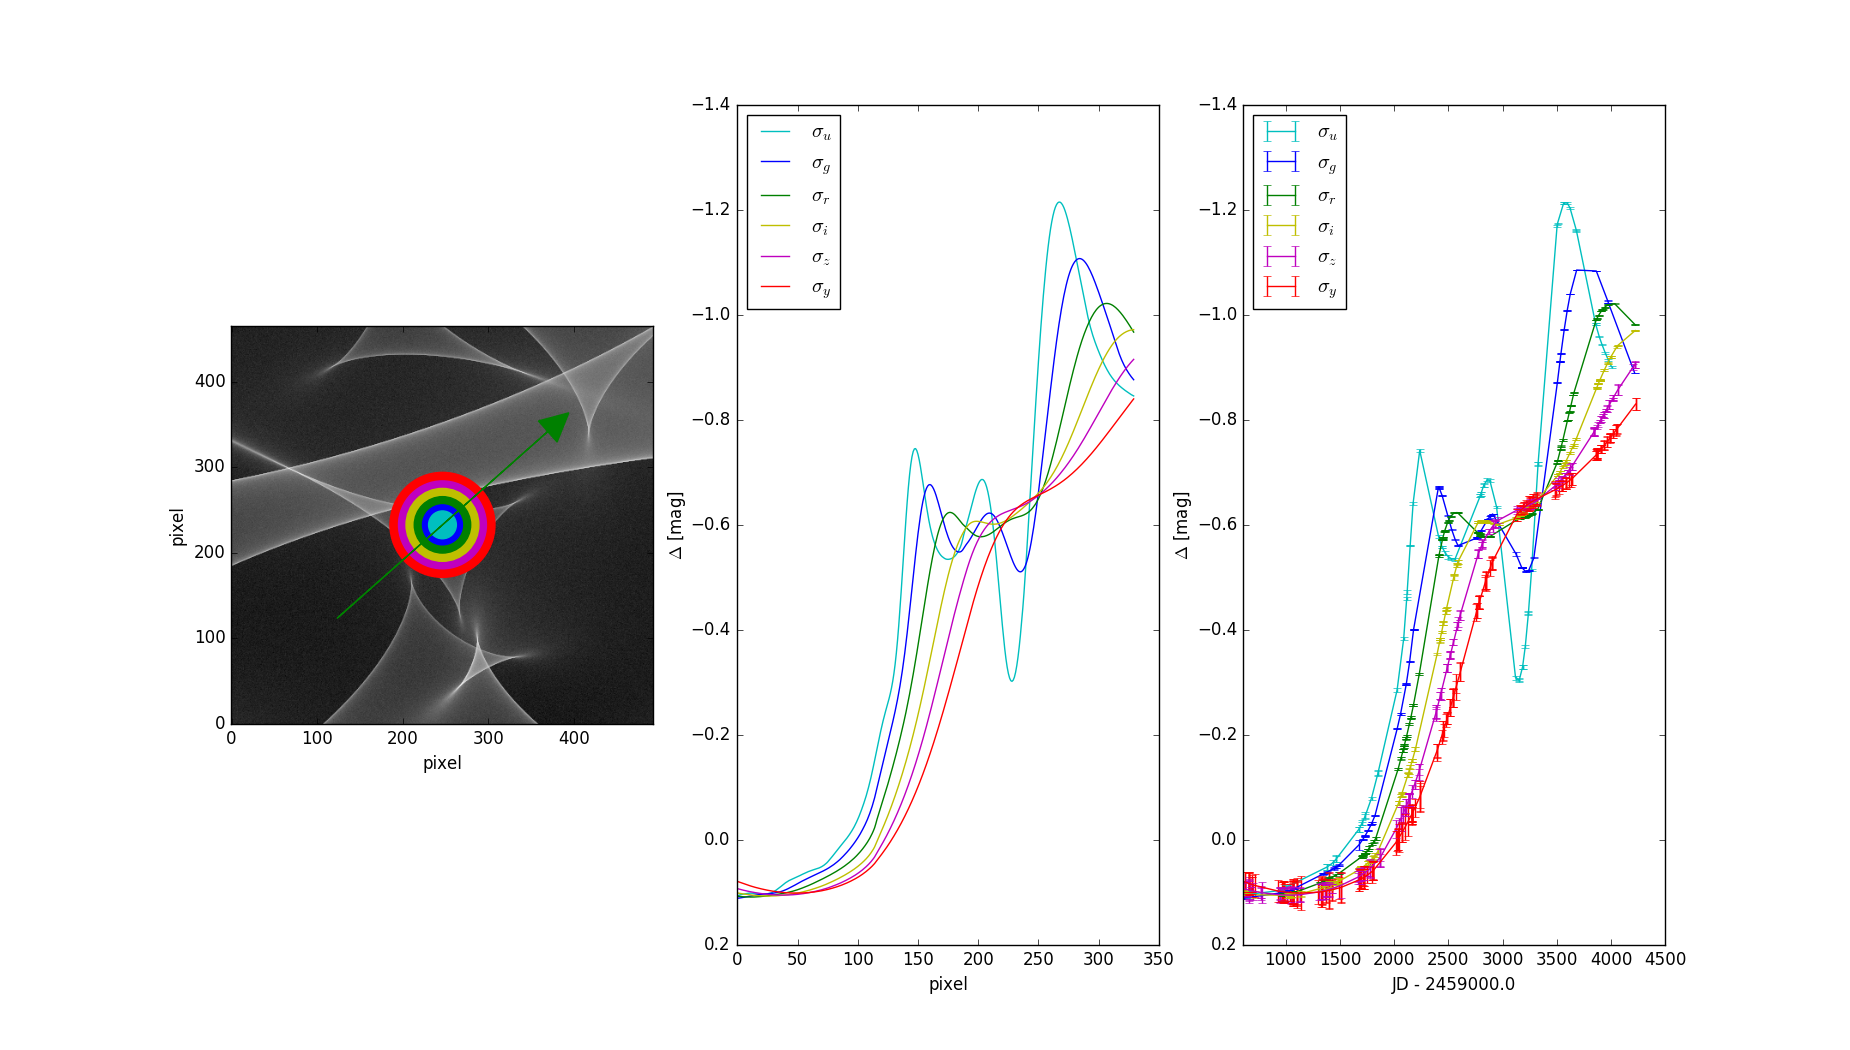
\includegraphics[width=\textwidth]{figs/agn/sim_ex.png}
		\caption{Ten year long simulated light curve for image A of RXJ1131-1231 using $\sigma_0$=2.0 light days at 2000\AA{}, $\alpha$=0.75, $\kappa$=0.494, $\gamma$=0.562 and 40\% of matter in compact form (stars). The left panel shows the concentric Gaussian emission regions observed by the LSST filters projected on top of the magnification pattern. The center panel shows the light curves with a ``perfect'' cadence. The right panel shows the magnitude values interpolated at epochs observed by LSST at the location of the system according the the ``Baseline Cadence'' (\opsimdbref{db:baseCadence})) Opsim output. The quasar was assumed to have the same intrinsic brightness in each band for easier comparison of variations between bands.}
		\label{microsimcurve}
	\end{figure}
\end{center}

% --------------------------------------------------------------------

\subsection{Metrics}
\label{sec:\secname:metrics}

Metrics for these section need to be defined by using simulated light curves
that take into account the several parameters that come into play in quasar
microlensing. These include: the time gap between visits in the same band,
projected CMB velocity, simulated peculiar velocities and redshifts of lenses
and sources as well as ``macro'' lens model parameters (i.e., surface mass
density and shear projected on top of lensed quasar images). Two metrics are
currently in consideration:

High Magnification Events recovery metric: This metric will measure the
number of high-magnification events recovered/missed considering the
cadence and season length in every LSST band and as the precision of the
brightness measurement.



Accretion disk size and slope metric: This metric will do a full
analysis of the ``pure'' microlensing light curves to recover these two
physical AGN parameters. The figure of merit would be the accuracy of
the measurement.

Since the microlensing signal can only be obtained after time delays between images
have been measured, both metrics need close interaction with time delay
measurements. As such, the ``Time Delays Challenges'' (see
\autoref{sec:lenstimedelays}) will include complete microlensing signal
simulations which also take into account the aforementioned parameters. Note
that given
the dependence on individual filter cadence and season length as well as
projected CMB velocities, every region on the sky needs to be considered
independently. Time Delay Challenge submissions will thus include recovered
``pure'' microlensing
light curves in addition to measured time-delays. By doing the reverse
procedure, i.e. using these ``pure'' microlensing light curves to statistically
re-obtain the input accretion disk sizes and thermal slopes, we will be able to
quantitatively measure the accuracy of the intrinsic accretion disk parameter
estimations for a given survey strategy.



We have build a preliminary tool that extracts micro lensing light curves from source plane magnification patterns as will be observed by LSST, taking into account:
\begin{itemize}
\item Projected peculiar velocities of the observer (projected CMB dipole in the direction of the system), lens and source.
\item Bulk motion of stars in the lensing galaxy (from the stellar velocity dispersion of the lens).
\item Specific LSST observing epochs in the direction of the system (from Opsim outputs).
\item Thermal profile slope of the accretion disk $\alpha$.
\item Scale size of the accretion disk $\sigma_{0}(\lambda)$ at a given wavelength $\lambda$.
\item Smooth (dark matter) to compact (stars) matter ratio on top of lensed quasar images.
\item ��Macro'' lens model parameters on top of lensed quasar images: Surface mass density $\kappa$ and shear $\gamma$.
\end{itemize}

\noindent In its current state, the tool assumes simple face-on concentric Gaussian emission regions for the accretion disk. An example of such a curve is shown in figure \ref{microsimcurve}. To recover the figure of merit, (measurement accuracy of $\alpha$ and $\sigma_0$), light curves generated with this tool for a given realistic lensed quasar system ($\kappa$, $\gamma$, $s$ and velocity dispersion of the lensing galaxy as well as time delays between lensed images) for every region in the sky need to analyzed using the above mentioned statistical analyses to recover the input accretion disk parameters.


% microlensing - convolve microlensing timescales for QSOs we already know
% about. how many of the high magnification events do we get? How bright?
% @tanguita

% --------------------------------------------------------------------

\subsection{OpSim Analysis}
\label{sec:\secname:analysis}

Much like the cosmology with lensed quasar time delays, we expect a strong
dependence of the proposed metrics with night-to-night cadence, uniformity and
season length. Maximizing these will maximize the likelihood of recovering high
magnification events, which in turn will provide the most stringent constraints
on
accretion disk structure. As mentioned above, since shorter wavelengths show
faster and stronger magnification events, in an ideal scenario, bluer bands would have
tighter night-to-night cadence.

\begin{center}
	\begin{figure}[hbt]
		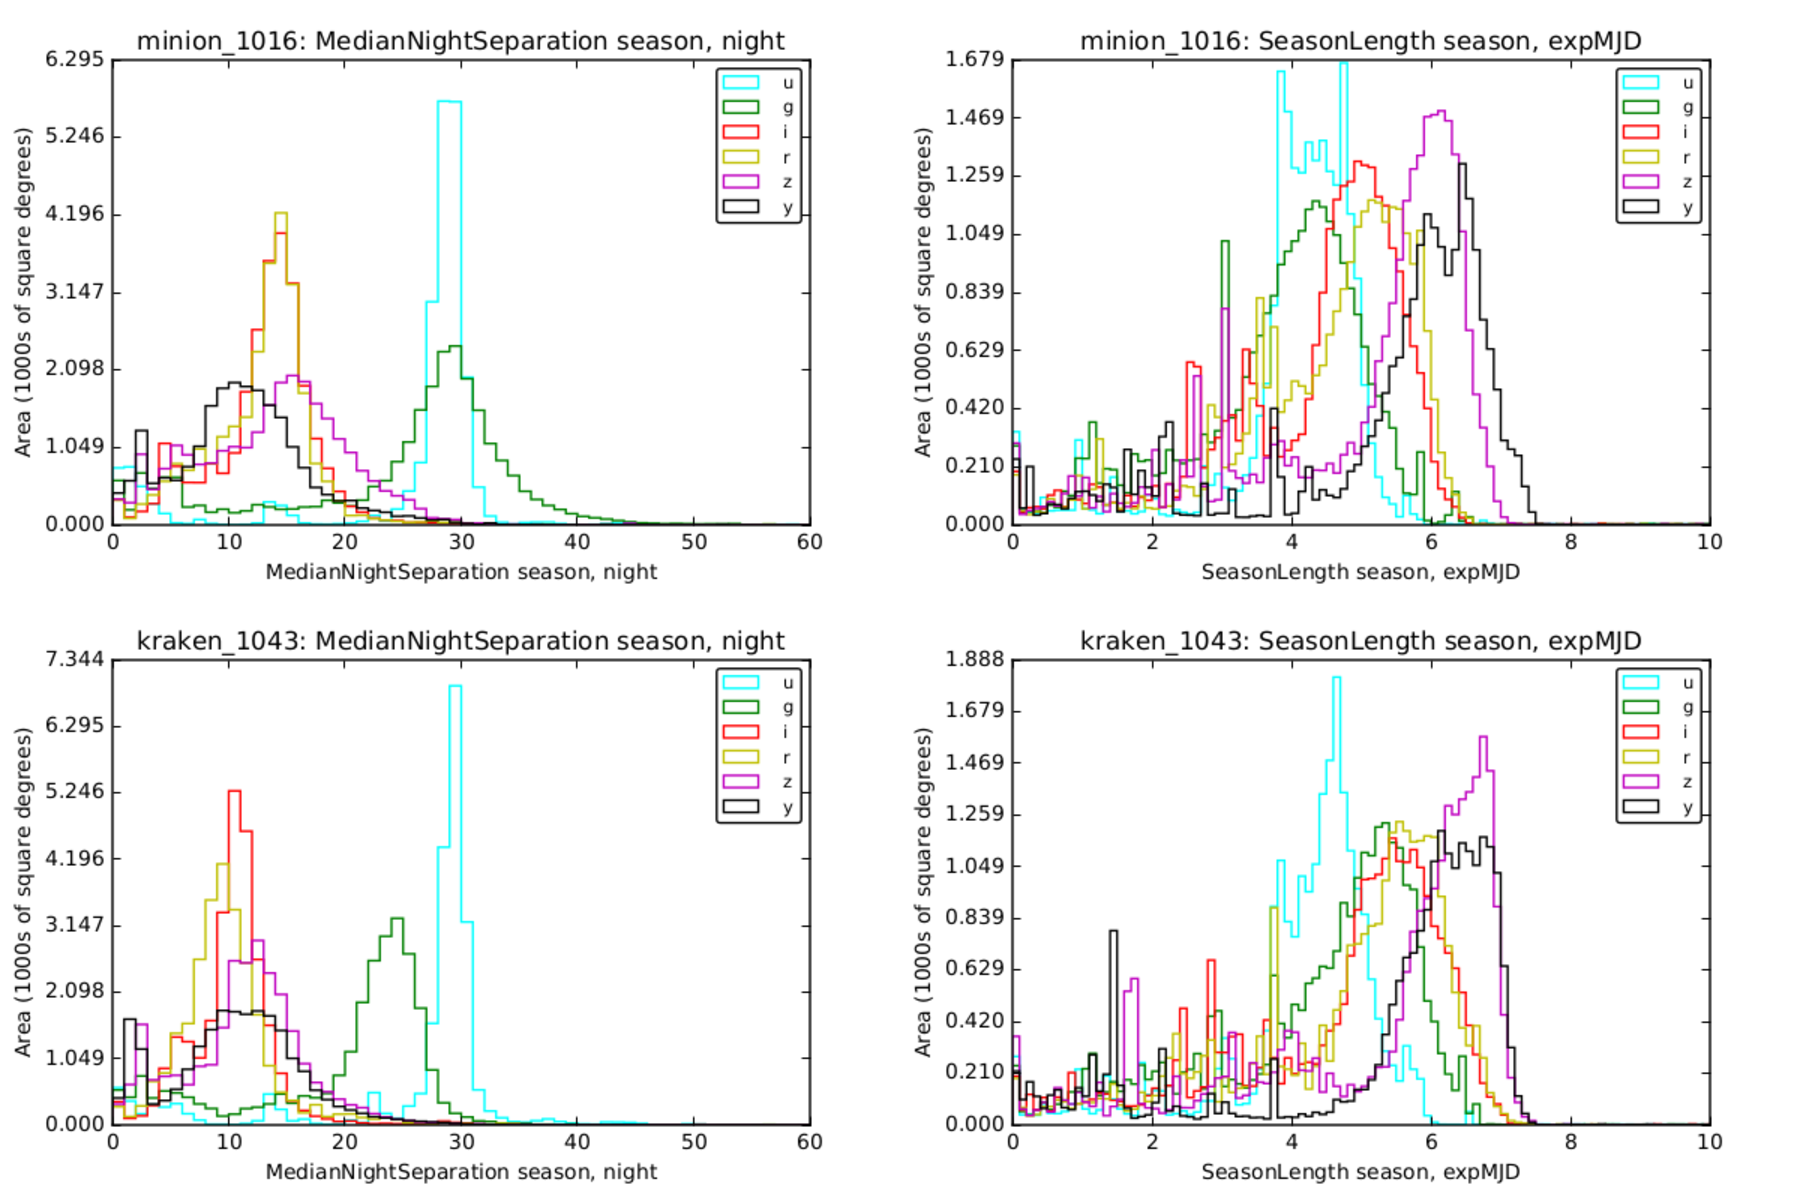
\includegraphics[width=\textwidth]{figs/agn/NightSep_seasonLength.pdf}
		\caption{Median Night Separation in days (left) and median season length in months (right) for all bands in the current ``Baseline Cadence'' (\opsimdbref{db:baseCadence}, top) and ``No Visit Pairs''	(\opsimdbref{db:NoVisitPairs}, bottom) opsim outputs.}
		\label{microfig}
	\end{figure}
\end{center}

As shown in figure \ref{microfig}, it seems there is a slightly better prospect
for the AGN structure with microlensing science case using the ``No Visit Pairs'' observing
strategy in comparison to the baseline strategy due to the smaller inter-night
gaps and longer season lengths in the g band. In both cases the night-to-night
cadence in the longer wavebands are compatible with the detection of most
microlensing events. On the other hand, in the u and g bands in both survey strategies it might compromise the results. Furthermore, in all LSST bands the spread in the night-to-night cadence (uniformity) and season length will likely dominate the uncertainties.

\begin{center}
	\begin{figure}[hbt]
		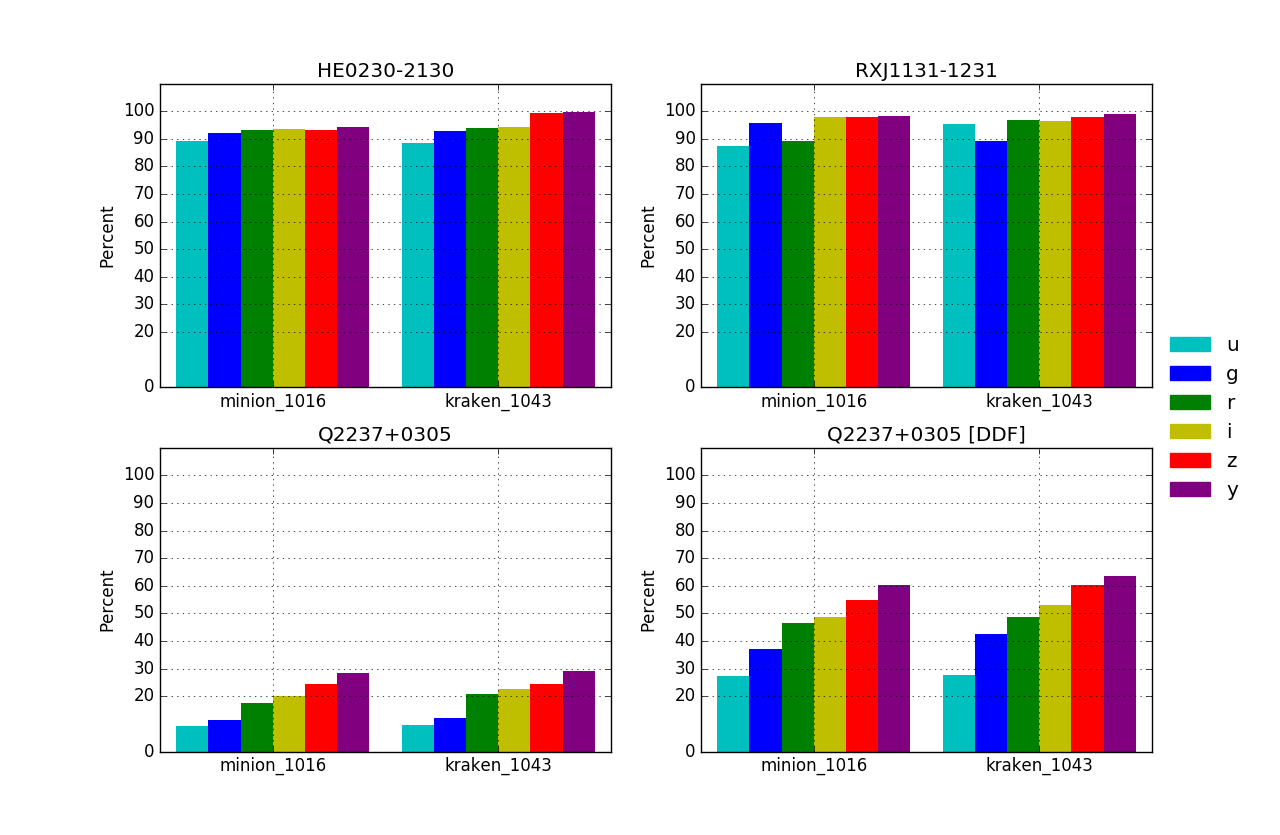
\includegraphics[width=\textwidth]{figs/agn/ulens_sim.png}
		\caption{Relative brightness fluctuations seen by LSST compared to ``perfect'' cadence for four systems as described in the text. The current ``Baseline Cadence'' (\opsimdbref{db:baseCadence}) and ``No Visit Pairs''	(\opsimdbref{db:NoVisitPairs}) opsim outputs are shown.All systems assumed to have accretion disk parameters of $\sigma_0$=2.0 light days and $\alpha$=0.75. Ratios are the median of 10000 simulated light curves.}
		\label{ulens_sim}
	\end{figure}
\end{center}


Given the nature of the commonly used statistical analyses to constrain the structure of accretion disk (accretion disk and slope metric), the accuracy of the recovery of the parameters will depend on the amount of brightness variations seen in the light curves even if no high-magnification events are seen. As a first assessment, we have used the light curve simulation tool outlined above to generate 10000 light curves for images A of three well known lensed systems where microlensing has been studied: RXJ1131-1231, HE0230-2130 and Q2237+0305. Additionally, given the very fast time scales expected for Q2237+0305 due to the relative redshifts of the source and lens, we also generate 10000 light curves for this system as if it was located in one of the LSST Deep Drilling Fields. All systems where assumed to have a size ($\sigma_0$) and slope ($\alpha$) parameters of 2.0 light days at $\lambda$=2000\AA{} and 0.75, respectively. Even when this experiment does not yield our proposed figure of merit, it does allow the comparison of the relative performance of different observing strategy regarding microlensing signal recovery.

The results of this experiment are shown in Figure \ref{ulens_sim}. For this analysis, at least for the four systems studied, we can see that even when the ``No Visit Pairs'' observing strategy shows a slightly better prospect compared to the ``Baseline Cadence'' for our science case, the difference is negligible. Note also that with the exception of Q2227+0305 (due to its very short time scales), both observing strategies will be able to map the expected microlensing induced brightness variations at a very high rate. It is important to consider that this is an optimistic analysis because the photometric uncertainties (including the dominating ones that come from the intrinsic variability correction from time delay measurements) have not been taken into account.


\subsection{Conclusions}
\label{sec:\secname:questions}

Here we answer the ten questions posed in
\autoref{sec:intro:evaluation:caseConclusions}:

\begin{description}

\item[Q1:] {\it Does the science case place any constraints on the
tradeoff between the sky coverage and coadded depth? For example, should
the sky coverage be maximized (to $\sim$30,000 deg$^2$, as e.g., in
Pan-STARRS) or the number of detected galaxies (the current baseline
of 18,000 deg$^2$)?}

\item[A1:] Given that lensed quasars are rare, maximizing the area
coverage would increase the number of systems to study. Even if this
comes at a cadence cost given that in most cases the studied OpSim
experiments provide sufficient temporal constraints.

\item[Q2:] {\it Does the science case place any constraints on the
tradeoff between uniformity of sampling and frequency of  sampling? For
example, a rolling cadence can provide enhanced sample rates over a part
of the survey or the entire survey for a designated time at the cost of
reduced sample rate the rest of the time (while maintaining the nominal
total visit counts).}

\item[A2:] Given the long timescales of microlensing events and the inability of predicting high-magnification events, uniform sampling would be better.

\item[Q3:] {\it Does the science case place any constraints on the
tradeoff between the single-visit depth and the number of visits
(especially in the $u$-band where longer exposures would minimize the
impact of the readout noise)?}

\item[A3:] No.

\item[Q4:] {\it Does the science case place any constraints on the
Galactic plane coverage (spatial coverage, temporal sampling, visits per
band)?}

\item[A4:] Not really, however, minimizing the coverage of the Galactic would benefit all AGN science cases.

\item[Q5:] {\it Does the science case place any constraints on the
fraction of observing time allocated to each band?}

\item[A5:] Ideally, shorter wavelengths should get denser (uniform) sampling.

\item[Q6:] {\it Does the science case place any constraints on the
cadence for deep drilling fields?}

\item[A6:] As in the main survey, AGN microlensing would benefit if the deep drilling fields observations would span long timescales with uniform coverage.

\item[Q7:] {\it Assuming two visits per night, would the science case
benefit if they are obtained in the same band or not?}

\item[A7:] Not very important for our since case. Given a choice, different bands would be better.

\item[Q8:] {\it Will the case science benefit from a special cadence
prescription during commissioning or early in the survey, such as:
acquiring a full 10-year count of visits for a small area (either in all
the bands or in a  selected set); a greatly enhanced cadence for a small
area?}

\item[A8:] No.

\item[Q9:] {\it Does the science case place any constraints on the
sampling of observing conditions (e.g., seeing, dark sky, airmass),
possibly as a function of band, etc.?}

\item[A9:] Seeing and Airmass are directly related to the ability to
accurately separate the flux from possibly blended lensed images. As
with most transient science cases, excellent seeing images are required
as templates for image substraction.

\item[Q10:] {\it Does the case have science drivers that would require
real-time exposure time optimization to obtain nearly constant
single-visit limiting depth?}

\item[A10:] No.

\end{description}


% % --------------------------------------------------------------------
%
% \subsection{Discussion}
% \label{sec:\secname:discussion}
%
% %Discussion: what risks have been identified? What suggestions could be
% %made to improve this science project's figure of merit, and mitigate
% %the identified risks?
%
%
% ====================================================================

\navigationbar
